\documentclass[ngerman,12pt]{article}

% PACKAGES
\usepackage{times}
\usepackage[ngerman]{babel}
\usepackage[utf8]{inputenc}
\usepackage[T1]{fontenc}
%\usepackage[latin1]{inputenc}
%\usepackage{eule}
%\usepackage{mpilogo}
\usepackage{url}
\usepackage{a4}
\usepackage{amsfonts}
\usepackage[usenames]{color}
\usepackage{verbatim}
\usepackage{graphicx}
\usepackage{hyperref}  % Marjan
\usepackage{listings}  % Marjan
\usepackage{booktabs}  % Marjan
\usepackage{dsfont}        % Symbol R for real numbers
\usepackage{color}

% PAGE LAYOUT
\setlength{\textwidth}{174mm}
\setlength{\textheight}{220mm}
\setlength{\topmargin}{10mm}
\setlength{\oddsidemargin}{10mm}
\setlength{\hoffset}{0mm}
\setlength{\voffset}{0mm}
\setlength{\parindent}{0mm}
\setlength{\parskip}{2mm}
\pagestyle{empty}

% EXERCISE SHEET SPECIFIC MAKROS
\renewcommand{\title}[1]{\par\vspace{5mm}\centerline{\Large #1}}
\newcommand{\subtitle}[1]{\par\vspace{1mm}\centerline{\footnotesize #1}\par}
\newcommand{\exercise}[1]{\par\vspace{3mm}{\bf Exercise{\hspace{1mm}}#1}\hspace{1mm}}
\newcommand{\extraexercise}[1]{\par\vspace{3mm}{\bf Bonus exercise{\hspace{1mm}}#1}\hspace{1mm}}
\newcommand{\examtask}[1]{\par\newpage{\bf Exemplary examination question{\hspace{1mm}}#1}\hspace{1mm}}
\newcommand{\examtasksolution}[1]{\par\vspace{5mm}{\bf Solution for Task{\hspace{1mm}}#1}\hspace{1mm}}
\newcommand{\points}[1]{\hspace{1mm}(#1 Punkte)\hspace{1mm}}
\newcommand{\TODO}[1]{{\sf [#1]}}

% GENERALLY USEFUL MATH MAKROS
\def\ceil#1{{\left\lceil#1\right\rceil}}
\def\floor#1{{\left\lfloor#1\right\rfloor}}
\def\mod{\mbox{ mod }}
\def\div{\mbox{ div }}
\def\sm{\backslash}
\def\IN{\mathbb{N}}
\def\IZ{\mathbb{Z}}
\def\IR{\mathbb{R}}
\def\Oh#1{O\left(#1\right)}
\def\Om#1{\Omega\left(#1\right)}
\def\Th#1{\Theta\left(#1\right)}
\def\eps{\varepsilon}

\begin{document}

% HEAD OF EXERCISE SHEETS
\setlength{\textwidth}{16.5cm}
\setlength{\textheight}{22cm}
\setlength{\topmargin}{0cm}
\setlength{\oddsidemargin}{-0.3cm}
\setlength{\evensidemargin}{0cm}
\vspace*{-20mm}

% Links der Name des Lehrstuhls.
\parbox{40mm}{%
%% LS für Algorithmen\\[0.2mm]
\footnotesize
\makebox[40mm][l]{Bioinformatics Group}\\[0.5mm]
Prof.~Dr. Backofen\\
Dr. Florian Eggenhofer\\[0.3mm]
Michael Uhl
} %\\[0.3mm]
% In der Mitte der Name der Veranstaltung.
\parbox{100mm}{\vspace*{1mm}\begin{center}\large\bf%
Algorithms and Data Structures\\[0mm]
WS 2016 / 2017\\[0mm]%
% \large\rm WS 2009/2010\\[0.5mm]%
{\footnotesize\rm \url{http://www.bioinf.uni-freiburg.de/Lehre/}}%
\end{center}}
\par\vspace{-5mm}
% Grauer Strich und rechts das Uni-Logo.
\definecolor{freiburg-gray}{rgb}{0.68,0.68,0.68}
\vspace*{2mm}
\raisebox{1.19cm}{%
\textcolor{freiburg-gray}{\rule{0.885\textwidth}{1.1mm}}}
% \textcolor[freiburggray]{0.6}{\rule{0.885\textwidth}{1.1mm}}}
% \textcolor[gray]{0.6}{\rule{0.05\textwidth}{1.1mm}}
% \raisebox{-0.5mm}{\begin{scriptsize}\quad \textsf{Lehrstuhl f\"ur Rechnerarchitektur}\quad\end{scriptsize}}
% \textcolor[gray]{0.6}{\rule{0.45\textwidth}{1.1mm}}}
\par\vspace*{-37.84mm}
\hspace*{\fill}\includegraphics[scale=0.49]{uni_logo.png}
% \hspace*{\fill}\includegraphics[scale=1.1]{unilogo_new}
\par\vspace{-5mm}

% \parbox{40mm}{\vspace*{-0mm}\includegraphics[width=40mm]{mpilogo-inf-compact}}
% %\parbox{40mm}{\vspace*{-3mm}\logo{40mm}}
% % course name etc. in the middle with some space left and right
% \hspace*{4mm}
% \parbox{100mm}{\vspace*{0mm}\begin{center}\Large\bf%
% Searching with Suffix Arrays\\[2mm]%
% \large\rm Bast, Majumdar, Weber \quad WS 2006/2007\\[0.5mm]%
% {\footnotesize\rm \url{http://www.mpi-inf.mpg.de/~bast/ir-seminar-ws06}}%
% \end{center}}
% \hspace*{3mm}
% % uni-sb owl to the right
% \parbox{27mm}{\eule[27mm]} %\\{\small FR 6.2 Informatik}
% % and at the bottom: a horizontal line, followed by some free space 
% \par\rule{\textwidth}{0.1mm}
% \bigskip


\title{Solutions Exercise Sheet 1}

\bigskip

\renewcommand{\baselinestretch}{1.1}\normalsize

\exercise{2} \\[10pt]
The following min heap is given in array representation:
\begin{center}
  \begin{tabular}{|c|c|c|c|c|c|c|c|c|c|c|c|c|c|c|c|c|}
    \hline
     1 & 6 & 2 & 4 & 7 & 3 & 9 & 11 & 13 & 12 & 14 & 5 & 15 & 8 & 10 & 13 & 13 \\
    \hline
  \end{tabular}
\end{center}

The corresponding tree diagram (edges marked red indicate violation of the heap properity):
\begin{figure}[htbp]
	\centering
	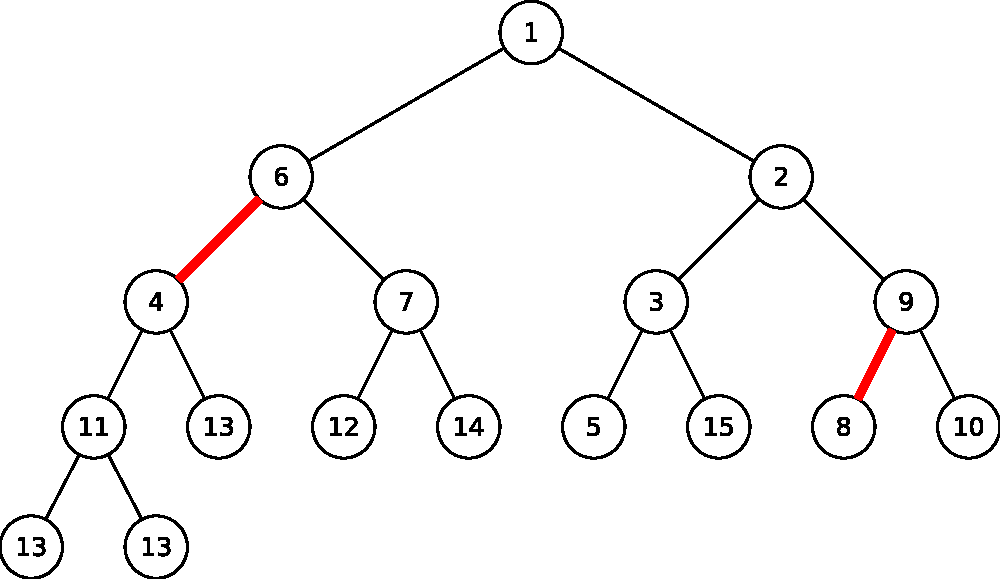
\includegraphics[width=0.7\textwidth]{images/A1_1}
\end{figure}

\newpage
Repaired heap:
\newline
\begin{figure}[htbp]
	\centering
	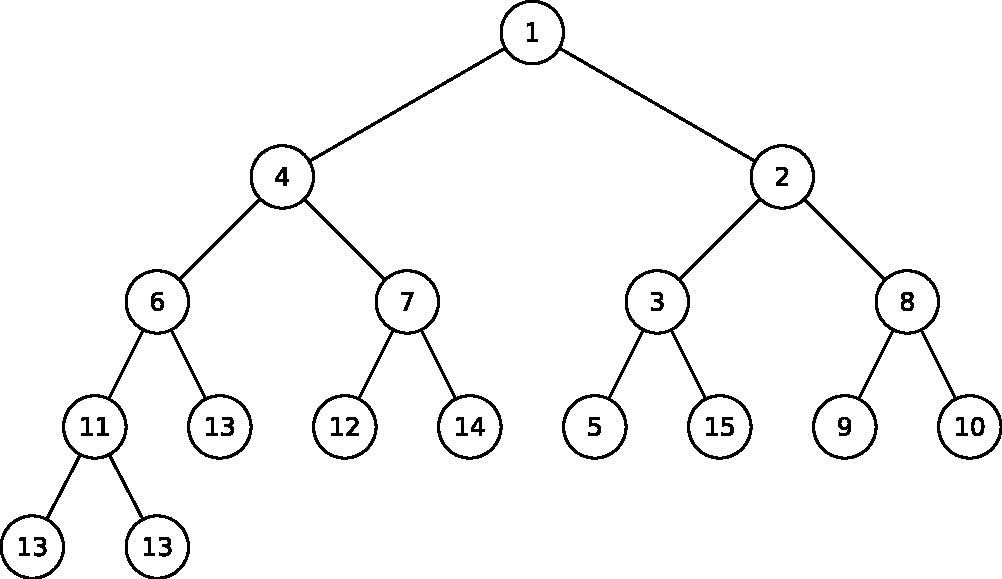
\includegraphics[width=0.7\textwidth]{images/A1_2}
\end{figure}

\end{document}
